\documentclass{exam}
\usepackage[utf8]{inputenc}
\usepackage{lmodern}
\usepackage{microtype}

% \usepackage[parfill]{parskip}
\usepackage[dvipsnames]{xcolor}
\usepackage{amsmath}
\usepackage{amsfonts}
\usepackage{amsthm}
\usepackage{siunitx}
\DeclareSIUnit\year{yr}
\DeclareSIUnit\foot{ft}
\DeclareSIUnit\litre{\liter}

\usepackage{skull}

\usepackage{pgfplots}
\usepgfplotslibrary{polar}
\pgfplotsset{compat=1.11}
\usepgfplotslibrary{statistics}
\usepackage{graphicx}
\usepackage{sidecap}
\sidecaptionvpos{figure}{c}
\usepackage{float}
\usepackage{gensymb}
\usepackage{tkz-euclide}
\usetkzobj{all}
\usepackage{commath}
\usepackage{hyperref}
\usepackage{enumitem}
\usepackage{wasysym}
\usepackage{multicol}
\usepackage{mathtools}
\usepackage{tcolorbox}
\usepackage{tabularx}
\usepackage[version=4]{mhchem}
\usepackage{changepage}
\usepackage{listings}
\lstset{basicstyle=\ttfamily\linespread{0.8}\small}

\renewcommand*{\thefootnote}{\fnsymbol{footnote}}

\newtheorem*{thm}{Theorem}
\newtheorem*{iden}{Identity}
\newtheorem*{lemma}{Lemma}
\newtheorem{obs}{Observation}
\theoremstyle{definition}
\newtheorem*{defn}{Definition}
\newtheorem*{ex}{Example}
\newtheorem{con}{Construction}
\newtheorem*{alg}{Algorithm}

\newtheoremstyle{break}
  {\topsep}{\topsep}%
  {\itshape}{}%
  {\bfseries}{}%
  {\newline}{}%
\theoremstyle{break}
\newtheorem*{bthm}{Theorem}

% russian integral
\usepackage{scalerel}
\DeclareMathOperator*{\rint}{\scalerel*{\rotatebox{17}{$\!\int\!$}}{\int}}

% \DeclareMathOperator*{\rint}{\int}

\pgfplotsset{vasymptote/.style={
    before end axis/.append code={
        \draw[densely dashed] ({rel axis cs:0,0} -| {axis cs:#1,0})
        -- ({rel axis cs:0,1} -| {axis cs:#1,0});
    }
}}

% \pointsinrightmargin
\boxedpoints
\pointname{}

\newcommand{\questioA}{\question[\texttt{\textbf{\color{Cerulean} A}}]}
\newcommand{\questioM}{\question[\texttt{\textbf{\color{PineGreen} M}}]}
\newcommand{\questioE}{\question[\texttt{\textbf{\color{WildStrawberry} E}}]}
\newcommand{\questioS}{\question[\texttt{\textbf{\color{Goldenrod} S}}]}
\newcommand{\questioO}{\question[\texttt{\textbf{\color{BurntOrange} O}}]}

\newcommand{\parA}{\part[\texttt{\textbf{\color{Cerulean} A}}]}
\newcommand{\parM}{\part[\texttt{\textbf{\color{PineGreen} M}}]}
\newcommand{\parE}{\part[\texttt{\textbf{\color{WildStrawberry} E}}]}
\newcommand{\parS}{\part[\texttt{\textbf{\color{Goldenrod} S}}]}
\newcommand{\parO}{\part[\texttt{\textbf{\color{BurntOrange} O}}]}

\newcommand{\subparA}{\subpart[\texttt{\textbf{\color{Cerulean} A}}]}
\newcommand{\subparM}{\subpart[\texttt{\textbf{\color{PineGreen} M}}]}
\newcommand{\subparE}{\subpart[\texttt{\textbf{\color{WildStrawberry} E}}]}
\newcommand{\subparS}{\subpart[\texttt{\textbf{\color{Goldenrod} S}}]}
\newcommand{\subparO}{\subpart[\texttt{\textbf{\color{BurntOrange} O}}]}

\newcommand{\mainHeader}[2]{\section*{NCEA Level 2 Mathematics\\#1. #2}}
\newcommand{\mainHeaderHw}[2]{\section*{NCEA Level 2 Mathematics (Homework)\\#1. #2}}
\newcommand{\seealso}[1]{\begin{center}\emph{See also #1.}\end{center}}
\newcommand{\drills}[1]{\begin{center}\emph{Drill problems: #1.}\end{center}}
\newcommand{\basedon}[1]{\begin{center}\emph{Notes largely based on #1.}\end{center}}


\begin{document}

\mainHeaderHw{15}{Kinematics and Rates of Change}
\subsection*{Reading}
\begin{center}
\begin{tcolorbox}[width=0.8\textwidth,colback={white},title={\textbf{Go and watch...}},colbacktitle=black,coltitle=white]
  \textcolor{black}{\url{https://www.youtube.com/watch?v=pI62ANEGK6Q}}
\end{tcolorbox}
\end{center}

\begin{center}
  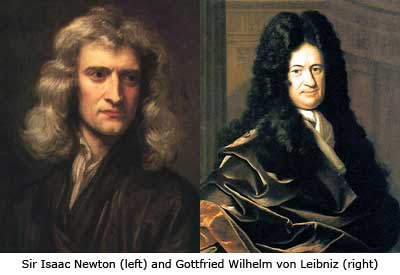
\includegraphics[width=0.5\textwidth]{newton-leibniz}

  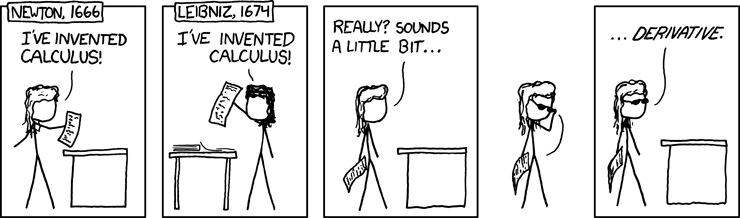
\includegraphics[width=0.6\textwidth]{newton-leibniz-2}\\
  \small{\url{https://xkcd.com/626/}}
\end{center}

The ancient Greeks used some of the ideas of calculus to calculate areas and volumes of
objects: for example, Archimedes (c. 287 -- 212 BC) used a limiting process to calculate the area of
a circle. The Greeks also considered some of the philosophical problems with these kinds of limiting
processes, some of which were not solved until the time of Cauchy in the 18th and 19th centuries.

The modern development of calculus is usually credited to Gottfried~Leibniz (1946 -- 1716)
and Isaac~Newton (1642 -- 1727), who independently developed coherent theories of calculus at the
turn of the 18th century. Both claimed scientific priority: Newton claimed to have begun development
of his theory in 1666 as part of his investigations into the laws of motion, but did not publish it
until after Leibniz began publishing in 1684.

Some argue that the resulting fallout between the followers of the Englishman, Newton, and the followers
of the German, Leibniz, set English mathematics back by decades compared to Europe.

\clearpage
\subsection*{Questions}
All distances are given in \si{\metre}, and all times in \si{\second}, unless otherwise stated.
\begin{questions}
  \question A particle moves in space along a single axis, with velocity function $ v(t) = t^2 + t - 12 $ (where $ t $ is measured from some
            arbitrary starting point).
    \begin{parts}
      \part What is the acceleration of the particle at $ t = \SI{10}{\second} $?
      \part The particle is closest to the origin at $ t = \SI{3}{\second} $.
        \begin{subparts}
          \subpart By considering $ v(t) $, show that $ t = 3 $ is indeed a turning point for the graph of the position function $ x(t) $ of the particle.
          \subpart If the minimum distance between the particle and the origin is \SI{300}{\metre}, calculate the distance from the particle
                   to the origin at $ t = \SI{10}{\second} $.
        \end{subparts}
    \end{parts}
  \question A cubic equation is a polynomial of degree three --- that is, a function
            of the form $ f(x) = ax^3 + bx^2 + cx + d $ where $ a \neq 0 $. Recall that
            a critical point is a point $ x $ where $ f'(x) = 0 $, or $ f'(x) $ is undefined.
            \begin{subparts}
              \subpart Sketch examples of a cubic function with zero, one, and two critical points.
              \subpart Prove that a cubic function can have a maximum of two critical points.
            \end{subparts}

\end{questions}

\end{document}
